 
 
  \chapter{ Les Serveurs}
 \section{Définitions}
 \begin{center}
	\begin{figure}[h]
		\hbox{ 
\includegraphics[width=0.5\textwidth]{PhotoMemoire/salle-serveur.jpg}}
		\caption{Une Salle Serveur}
	\end{figure}
\end{center}
\paragraph{ }
Les serveurs sont des ordinateurs ou des systèmes informatiques qui fournissent des services ou des ressources à d'autres ordinateurs ou utilisateurs sur un réseau. Ils peuvent être utilisés pour stocker des données, héberger des sites Web, exécuter des applications et bien plus encore. Il existe différents types de serveurs, tels que les serveurs de fichiers, les serveurs de messagerie, les serveurs de bases de données et les serveurs de jeux en ligne. Les serveurs sont souvent utilisés pour fournir des services à distance, ce qui permet aux utilisateurs d'y accéder à partir de n'importe où dans le monde.
 Dans ce point ci-après nous allons la plupart des sortes de serveurs les plus rependus 
 \subsection*{Fonctionnement}
 \paragraph{ }
 Le serveur fonctionne en réseau; Peu importe sa mission, il a pour fonction d’écouter les requêtes formulées par les ordinateurs clients et de les traiter s’il le peut, en communiquant une information ou en donnant accès à un logiciel ou un fichier à l’utilisateur qui en a besoin.\\
  Pour fonctionner correctement, le serveur doit être en mesure de vérifier certaines informations.\\
   Il est en effet configuré pour autoriser l’accès à une liste précise d’utilisateurs, sur des plages horaires définies ou à choisir qui peut lire, modifier ou supprimer des fichiers.\\
   Cela implique que chaque ordinateur client soit identifiable et puisse recevoir la réponse du serveur selon la méthode attendue.
 \subsection*{Rôles}
 
  \underline Stockage: Les serveurs stockent de grandes quantités de données, telles que des fichiers, des bases de données et des applications.\\
   Ces données sont accessibles aux utilisateurs ou à d'autres serveurs du réseau.
  Les serveurs peuvent effectuer des calculs complexes, tels que ceux nécessaires à la recherche scientifique ou à la modélisation financière.\\ Cela permet aux autres ordinateurs du réseau de se concentrer sur d'autres tâches.
  \paragraph{ }
   Les serveurs facilitent la communication entre les utilisateurs et les autres ordinateurs du réseau. Cela peut se faire par le biais du courrier électronique, du partage de fichiers ou de la navigation sur le web.\\
 
   Les serveurs peuvent assurer la sécurité du réseau, par exemple en authentifiant les utilisateurs et en cryptant les données.\\
 
 Outre ces rôles généraux, les serveurs peuvent être spécialisés dans des tâches spécifiques. Par exemple, un serveur web est un type de serveur qui héberge des sites web. Un serveur de base de données est un type de serveur qui stocke et gère des bases de données.\\
 
 Le rôle spécifique d'un serveur dépend des besoins du réseau. Cependant, tous les serveurs ont pour objectif commun de fournir des services aux autres ordinateurs du réseau.
 
 \subsection*{ Sortes De Serveur}
\begin{enumerate}
     \item Serveur Web
     \item Serveur de Messagerie
     \item Serveur de fichiers
     \item Serveur de base de données 
     \item Serveur d'applications
     \item Serveur de virtualisation
     \item Serveur DNS
     \item Serveur de sauvegarde 
     \item Serveur de jeu 
     \item Serveur de médias    
\end{enumerate}
 
  
\section{Les Serveurs Web}
 
\begin{figure}[h]
	\hbox{
	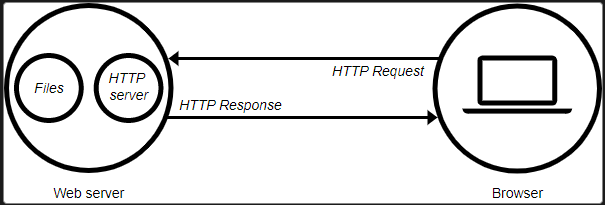
\includegraphics[width=0.5\textwidth]{PhotoMemoire/Server_web.png}}
\caption{Le Schéma d'un serveur Web}
\end{figure}
\paragraph{ }
Les serveurs Web sont des ordinateurs ou des programmes informatiques qui fournissent des pages Web aux clients qui les demandent via un navigateur Web. Ils sont utilisés pour héberger des sites Web et distribuer du contenu en ligne. Les serveurs Web peuvent exécuter différents types de logiciels, tels que Apache, Nginx, Microsoft IIS et bien d'autres. Les pages Web sont généralement créées en utilisant des langages de programmation Web tels que HTML, CSS et JavaScript. Les serveurs Web peuvent également exécuter des applications Web, telles que des forums en ligne, des blogs, des magasins en ligne et bien plus encore.

\subsection{Quelques vulnérabilités Sur Les Serveurs Web }
\paragraph{ }
Il y a plusieurs vulnérabilités qui peuvent affecter un serveur web, en voici quelques exemples :
\paragraph{ }
$\bullet$ Injection SQL : Cette vulnérabilité permet à un attaquant d'injecter du code SQL malveillant dans une requête pour détourner le contrôle de la base de données.
\paragraph{ }
$\bullet$ Cross-site scripting (XSS) : Cette vulnérabilité permet à un attaquant d'injecter du code malveillant dans une page Web pour voler des informations d'authentification ou d'autres données sensibles.
\paragraph{ }
$\bullet$ Vulnérabilités du serveur HTTP : Les serveurs HTTP tels que Apache, Nginx et IIS peuvent être vulnérables à des attaques telles que les dénis de service (DoS) et les dénis de service distribués (DDoS).
\paragraph{ }
$\bullet$ Mauvaise configuration : Une mauvaise configuration du serveur web peut permettre aux attaquants d'accéder aux fichiers sensibles ou d'exécuter du code malveillant.
\paragraph{ }
$\bullet$ Vulnérabilités du CMS : Les systèmes de gestion de contenu tels que WordPress et Drupal peuvent être vulnérables à des attaques telles que les injections SQL et les attaques de force brute.\\
\paragraph{ }
Il est important de mettre en place des mesures de sécurité adéquates pour protéger les serveurs web contre ces vulnérabilités potentielles, telles que la mise à jour régulière de la sécurité du système et l'utilisation de logiciels de sécurité pour détecter et prévenir les attaques potentielles. \\Les développeurs de sites web doivent également être conscients des meilleures pratiques de sécurité, telles que la validation des entrées utilisateur et l'utilisation de l'encodage pour se protéger contre les attaques XSS.\\


\section{Serveurs de Messageries}
	\begin{figure}[h]
		\hbox{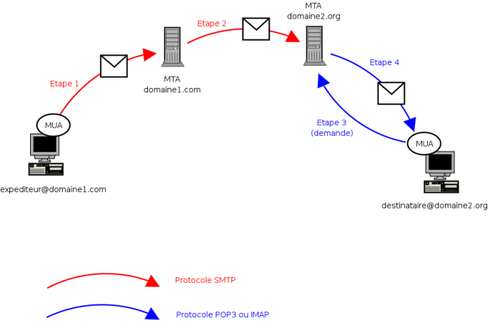
\includegraphics[width=0.8\textwidth]{PhotoMemoire/Serveur_Messagerie.png}}
\caption{Schéma d'un Serveur de Messagerie}
\end{figure}
\paragraph{ }

Un serveur de messagerie est un type de serveur qui est utilisé pour envoyer et recevoir des courriers électroniques (e-mails). Les serveurs de messagerie sont essentiels pour le fonctionnement du courrier électronique car ils sont responsables de la distribution des messages entre les différents utilisateurs.\\
\paragraph{ }
Il existe deux types principaux de serveurs de messagerie : le serveur SMTP (Simple Mail Transfer Protocol) et le serveur POP (Post Office Protocol).\\
\paragraph{ }
Le serveur SMTP est utilisé pour envoyer des courriers électroniques. Lorsqu'un utilisateur envoie un e-mail, le client de messagerie envoie le message au serveur SMTP, qui se charge de le transférer au serveur de messagerie du destinataire.\\

Le serveur POP est utilisé pour récupérer les courriers électroniques sur le serveur de messagerie. Les clients de messagerie utilisent le protocole POP pour se connecter au serveur de messagerie et récupérer les messages qui leur sont destinés.

Il existe également un autre protocole appelé IMAP (Internet Message Access Protocol) qui est utilisé pour accéder aux messages sur le serveur de messagerie sans les télécharger sur l'ordinateur local. IMAP permet aux utilisateurs de se connecter à leur boîte de réception depuis n'importe quel ordinateur ou appareil connecté à Internet.

Les serveurs de messagerie peuvent être configurés pour fournir des fonctionnalités supplémentaires telles que la sécurité des messages, la gestion des spams et des virus, la gestion des listes de diffusion, etc. Les serveurs de messagerie sont également souvent intégrés à des suites de collaboration pour permettre le partage de calendriers, de contacts, de tâches, etc.
\subsection{Quelques vulnérabilités Sur Les Serveurs de Messageries }
Il existe plusieurs vulnérabilités potentielles qui peuvent affecter les serveurs de messagerie. Voici quelques exemples :
\paragraph{ }
$\bullet$Injection de code : Les attaquants peuvent exploiter des vulnérabilités dans le serveur de messagerie pour injecter du code malveillant dans les e-mails, qui peuvent ensuite être utilisés pour exécuter des attaques de phishing, des attaques de logiciels malveillants ou d'autres types d'attaques.

\paragraph{ }
$\bullet$ Attaques de force brute : Les attaquants peuvent tenter de deviner les identifiants de connexion des utilisateurs en utilisant des attaques de force brute, qui impliquent l'utilisation de programmes pour tester toutes les combinaisons de noms d'utilisateur et de mots de passe possibles.

\paragraph{ }
$\bullet$ Attaques par déni de service (DoS) : Les attaquants peuvent lancer des attaques par déni de service (DoS) contre le serveur de messagerie pour le rendre indisponible, ce qui peut empêcher les utilisateurs d'accéder à leurs e-mails ou de les envoyer.

\paragraph{ }
$\bullet$Vulnérabilités de sécurité : Les serveurs de messagerie peuvent avoir des vulnérabilités de sécurité connues qui peuvent être exploitées par les attaquants pour accéder à des données sensibles, tels que des courriels confidentiels ou des informations d'identification.

\paragraph{ }
$\bullet$Vulnérabilités de configuration : Les serveurs de messagerie peuvent avoir des vulnérabilités de configuration qui peuvent être exploitées par les attaquants pour accéder à des données sensibles, tels que des listes de contacts, des calendriers et des tâches.
\paragraph{ }
Il est important de mettre en place des mesures de sécurité adéquates pour protéger les serveurs de messagerie contre ces vulnérabilités potentielles, telles que la mise à jour régulière de la sécurité du système et l'utilisation de logiciels de sécurité pour détecter et prévenir les attaques potentielles.\\
 Les utilisateurs doivent également être éduqués sur les meilleures pratiques de sécurité, telles que la création de mots de passe forts et l'utilisation de l'authentification à deux facteurs pour protéger leurs comptes de messagerie.\\
\section{Serveur de fichiers}
	\begin{figure}[h]
		\hbox{
	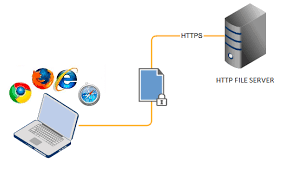
\includegraphics[width=0.8\textwidth]{PhotoMemoire/serveur_fichier.png}}
\caption{Schéma De Serveur De Fichier }
\end{figure}
\paragraph{ }
Un serveur de fichiers est un type de serveur qui stocke des fichiers et des dossiers, et permet à des utilisateurs de les accéder et de les partager via un réseau. Les serveurs de fichiers peuvent être configurés pour fournir différentes fonctionnalités, telles que :
\begin{enumerate}
 \item   Partage de fichiers : Les utilisateurs peuvent accéder aux fichiers stockés sur le serveur et les partager avec d'autres utilisateurs du réseau.
 
 \item Gestion des droits d'accès : Les administrateurs peuvent définir des autorisations d'accès pour chaque utilisateur ou groupe d'utilisateurs, afin de contrôler qui peut accéder à quels fichiers.
 
 \item Sauvegarde de données : Les serveurs de fichiers peuvent être configurés pour effectuer des sauvegardes régulières des fichiers stockés, afin de protéger les données contre la perte ou la corruption.
 
 \item Synchronisation de fichiers : Les utilisateurs peuvent synchroniser des fichiers entre le serveur de fichiers et leur ordinateur local, pour assurer une cohérence des données.
 
 \item Accès à distance : Les utilisateurs peuvent accéder aux fichiers stockés sur le serveur de fichiers à partir d'un emplacement distant en utilisant un client de connexion sécurisé.
 
  \item Stockage en nuage : Les serveurs de fichiers peuvent être configurés pour stocker des fichiers dans le cloud, ce qui permet aux utilisateurs d'y accéder à partir de n'importe où avec une connexion Internet.
 
\item Accès multiplateforme : Les serveurs de fichiers peuvent être configurés pour fournir un accès multiplateforme aux utilisateurs, ce qui permet aux utilisateurs d'accéder aux fichiers à partir de différents systèmes d'exploitation tels que Windows, Mac OS ou Linux.
 
\end{enumerate}
Les serveurs de fichiers sont couramment utilisés dans les entreprises pour stocker et partager des fichiers entre les employés, mais ils peuvent également être utilisés dans des environnements domestiques pour stocker et partager des fichiers entre les membres de la famille.
\subsection{Quelques vulnérabilités Sur Les Serveurs de Fichier}
Il existe plusieurs vulnérabilités potentielles qui peuvent affecter les serveurs de fichiers. Voici quelques exemples :

\begin{enumerate}
\item   Vulnérabilités de sécurité : Les serveurs de fichiers peuvent avoir des vulnérabilités de sécurité connues qui peuvent être exploitées par les attaquants pour accéder à des données sensibles, telles que des fichiers confidentiels ou des informations d'identification.
 
 \item   Vulnérabilités de configuration : Les serveurs de fichiers peuvent avoir des vulnérabilités de configuration qui peuvent être exploitées par les attaquants pour accéder à des données sensibles, telles que des fichiers de configuration ou des répertoires de fichiers.
 
 \item   Attaques par déni de service (DoS) : Les attaquants peuvent lancer des attaques par déni de service (DoS) contre le serveur de fichiers pour le rendre indisponible, ce qui peut empêcher les utilisateurs d'accéder aux fichiers hébergés sur ce serveur.
 
  \item  Attaques de force brute : Les attaquants peuvent tenter de deviner les identifiants de connexion des utilisateurs en utilisant des attaques de force brute, qui impliquent l'utilisation de programmes pour tester toutes les combinaisons de noms d'utilisateur et de mots de passe possibles.
 
 \item   Fuites de données : Les serveurs de fichiers peuvent être vulnérables aux fuites de données, qui peuvent se produire lorsque des données sensibles sont stockées de manière inappropriée ou lorsque des utilisateurs non autorisés y ont accès.
\end{enumerate}

 
\paragraph{ }
 
Il est important de mettre en place des mesures de sécurité adéquates pour protéger les serveurs de fichiers contre ces vulnérabilités potentielles, telles que la mise à jour régulière de la sécurité du système et l'utilisation de logiciels de sécurité pour détecter et prévenir les attaques potentielles.\\
 Les utilisateurs doivent également être éduqués sur les meilleures pratiques de sécurité, telles que la création de mots de passe forts et l'utilisation de l'authentification à deux facteurs pour protéger leur accès aux fichiers stockés sur le serveur de fichiers.
\section{Serveur de Base de Données }
	\begin{figure}[h]
		
		\hbox{
	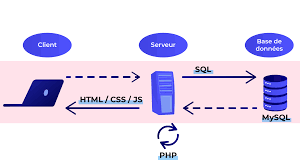
\includegraphics[width=0.8\textwidth]{PhotoMemoire/serveur_bdd.png}}
\caption{Schema De Serveur De Base De Données}
\end{figure}
\paragraph{ }
Un serveur de base de données est un type de serveur qui stocke des données et fournit des services pour gérer ces données. Il permet aux utilisateurs de stocker, d'organiser, d'accéder et de gérer des données de manière efficace et sécurisée.
\paragraph{ }
Les serveurs de base de données sont utilisés pour stocker des informations sur des produits, des clients, des transactions financières, des employés, des stocks, etc. Ils sont également utilisés pour alimenter des applications qui nécessitent un accès rapide et efficace aux données, telles que les sites web, les applications mobiles, les systèmes de gestion de la relation client (CRM), les systèmes de gestion de la chaîne d'approvisionnement (SCM), etc.

Les serveurs de bases de données peuvent être configurés pour fournir différentes fonctionnalités, telles que :

\begin{enumerate}
	
 \item Langage de requête : Les serveurs de bases de données prennent en charge des langages de requête tels que SQL (Structured Query Language) pour interroger et récupérer les données stockées.
 
 \item Gestion des transactions : Les serveurs de bases de données prennent en charge la gestion des transactions pour garantir l'intégrité des données et éviter les conflits.
 
 \item Gestion des utilisateurs et des droits d'accès : Les administrateurs peuvent définir des autorisations d'accès pour chaque utilisateur ou groupe d'utilisateurs, afin de contrôler qui peut accéder à quelles données.
 
  \item Sauvegarde et restauration : Les serveurs de bases de données peuvent être configurés pour effectuer des sauvegardes régulières des données stockées, afin de protéger les données contre la perte ou la corruption.
 
 \item Réplication des données : Les serveurs de bases de données peuvent être configurés pour répliquer les données sur plusieurs serveurs, pour améliorer la disponibilité et la redondance des données.
 
 \item Sécurité des données : Les serveurs de bases de données peuvent être configurés pour fournir des fonctionnalités de sécurité avancées, telles que le chiffrement des données, l'authentification à deux facteurs, etc.
 
\end{enumerate}
\paragraph{ }
Les serveurs de bases de données sont couramment utilisés dans les entreprises pour stocker et gérer des données importantes, mais ils peuvent également être utilisés dans des environnements domestiques pour stocker et gérer des données personnelles telles que les finances, les contacts, les photos, etc.

\subsection{Quelques vulnérabilités Sur Les Serveurs de Base De Donnes }

Il existe plusieurs vulnérabilités potentielles qui peuvent affecter les serveurs de bases de données. Voici quelques exemples :
\begin{enumerate}



	\item   Injection SQL : Les attaquants peuvent exploiter des vulnérabilités dans le serveur de base de données pour injecter du code SQL malveillant, qui peut permettre aux attaquants de prendre le contrôle du serveur de base de données, de modifier ou de supprimer des données, ou encore d'accéder à des informations confidentielles.
	
	\item   Vulnérabilités de sécurité : Les serveurs de bases de données peuvent avoir des vulnérabilités de sécurité connues, telles que la configuration par défaut de mots de passe faibles, qui peuvent être exploitées par les attaquants pour accéder à des données sensibles.
	
	\item   Attaques par déni de service (DoS) : Les attaquants peuvent lancer des attaques par déni de service (DoS) contre le serveur de base de données pour le rendre indisponible, ce qui peut empêcher les utilisateurs d'accéder aux données stockées sur ce serveur.
	
	\item   Vulnérabilités de configuration : Les serveurs de bases de données peuvent avoir des vulnérabilités de configuration qui peuvent être exploitées par les attaquants pour accéder à des données sensibles, telles que des informations de connexion ou des fichiers de configuration.
	
	\item   Fuites de données : Les serveurs de bases de données peuvent être vulnérables aux fuites de données, qui peuvent se produire lorsque des données sensibles sont stockées de manière inappropriée ou lorsque des utilisateurs non autorisés y ont accès.
\end{enumerate}
\paragraph{ }

Il est important de mettre en place des mesures de sécurité adéquates pour protéger les serveurs de bases de données contre ces vulnérabilités potentielles, telles que la mise à jour régulière de la sécurité du système et l'utilisation de logiciels de sécurité pour détecter et prévenir les attaques potentielles. Les développeurs de bases de données doivent également être conscients des meilleures pratiques de sécurité, telles que la validation des entrées utilisateur et l'utilisation de l'authentification à deux facteurs pour protéger l'accès aux données stockées sur le serveur de bases de données.
\section{Serveur d'Application}
	\begin{figure}[h]
		\hbox{
	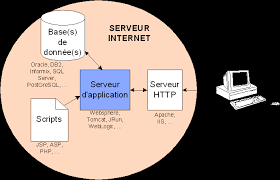
\includegraphics[width=0.8\textwidth]{PhotoMemoire/serveur_application.png}}
\caption{Schéma D'un serveur D'application}
\end{figure}
\paragraph{ }

Un serveur d'application est un type de serveur qui héberge des applications et fournit des services d'application aux clients. Les serveurs d'application sont essentiels pour les entreprises qui développent et déploient des applications commerciales, car ils fournissent une plateforme pour exécuter et gérer ces applications de manière efficace et sécurisée.
\paragraph{ }
Les serveurs d'application peuvent être utilisés pour héberger une grande variété d'applications, telles que les applications de commerce électronique, les applications de gestion de contenu, les applications de gestion de la relation client (CRM), les applications de gestion de la chaîne d'approvisionnement (SCM), les applications de collaboration, etc.

Les serveurs d'application peuvent fournir différentes fonctionnalités, telles que :
\begin{enumerate}
	 \item Gestion de la connectivité : Les serveurs d'application peuvent gérer la connectivité entre les applications et les différents systèmes d'information, tels que les bases de données, les systèmes de fichiers, les services web, etc.
	 
	 \item Gestion des transactions : Les serveurs d'application peuvent gérer les transactions pour garantir l'intégrité des données et éviter les conflits.
	 
	 \item Gestion de la sécurité : Les serveurs d'application peuvent fournir des fonctionnalités de sécurité avancées pour protéger les applications et les données contre les menaces potentielles.
	 
	 \item Gestion des sessions : Les serveurs d'application peuvent gérer les sessions pour assurer la continuité des services aux utilisateurs lorsqu'ils passent d'une page à l'autre ou lorsqu'ils se connectent à l'application à partir de différents appareils.
	 
	 \item Gestion des performances : Les serveurs d'application peuvent surveiller et optimiser les performances de l'application pour assurer une expérience utilisateur rapide et fluide.
	 
\end{enumerate}

\paragraph{ }
Les serveurs d'application sont souvent utilisés en conjonction avec d'autres outils de développement et de déploiement, tels que les serveurs web, les bases de données, les outils de développement intégrés (IDE), les systèmes de contrôle de version, etc.\\
\subsection{Quelques vulnérabilités Sur Les Serveurs d'Application }
Il existe plusieurs vulnérabilités potentielles qui peuvent affecter les serveurs d'application. Voici quelques exemples :
\begin{enumerate}
\item   Vulnérabilités de sécurité : Les serveurs d'application peuvent avoir des vulnérabilités de sécurité connues, telles que des failles dans les algorithmes de chiffrement ou des vulnérabilités dans les bibliothèques tierces, qui peuvent être exploitées par les attaquants pour accéder à des données sensibles ou prendre le contrôle du serveur.

\item   Attaques par déni de service (DoS) : Les attaquants peuvent lancer des attaques par déni de service (DoS) contre le serveur d'application pour le rendre indisponible, ce qui peut empêcher les utilisateurs d'accéder aux applications hébergées sur ce serveur.

\item   Injection de code : Les attaquants peuvent exploiter des vulnérabilités dans le serveur d'application pour injecter du code malveillant dans les applications, qui peuvent ensuite être utilisées pour exécuter des attaques de phishing, des attaques de logiciels malveillants ou d'autres types d'attaques.

\item  Vulnérabilités de configuration : Les serveurs d'application peuvent avoir des vulnérabilités de configuration qui peuvent être exploitées par les attaquants pour accéder à des données sensibles, telles que des informations de connexion ou des fichiers de configuration.

\item   Fuites de données : Les serveurs d'application peuvent être vulnérables aux fuites de données, qui peuvent se produire lorsque des données sensibles sont stockées de manière inappropriée ou lorsque des utilisateurs non autorisés y ont accès.
\end{enumerate}

\paragraph{ }

Il est important de mettre en place des mesures de sécurité adéquates pour protéger les serveurs d'application contre ces vulnérabilités potentielles, telles que la mise à jour régulière de la sécurité du système et l'utilisation de logiciels de sécurité pour détecter et prévenir les attaques potentielles.\\
 Les développeurs d'applications doivent également être conscients des meilleures pratiques de sécurité, telles que la validation des entrées utilisateur et l'utilisation de l'authentification à deux facteurs pour protéger les applications hébergées sur le serveur d'application.\\
 
 \section{Serveur DNS}
	\begin{figure}[h]
	\hbox{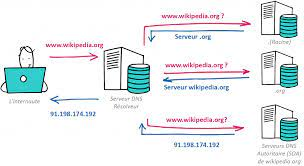
\includegraphics[width=0.8\textwidth]{PhotoMemoire/serveur_dns.jpeg}}
	\caption{Schéma d'un Serveur DNS}
\end{figure}
\paragraph{ }
Un serveur DNS (Domain Name System) est un type de serveur qui permet de traduire les noms de domaine en adresses IP. Les noms de domaine sont des identificateurs textuels, tels que "google.com" ou "facebook.com", qui sont plus faciles à mémoriser que les adresses IP numériques qui identifient les ordinateurs et les serveurs sur Internet.
\paragraph{ }
Lorsqu'un utilisateur entre un nom de domaine dans son navigateur web, le navigateur envoie une requête DNS au serveur DNS pour obtenir l'adresse IP correspondante. Le serveur DNS répond alors avec l'adresse IP, qui est utilisée pour établir la connexion avec le serveur web correspondant.
\paragraph{ }
Les serveurs DNS sont essentiels pour le fonctionnement d'Internet, car ils permettent aux utilisateurs d'accéder aux sites web et aux services en ligne en utilisant des noms de domaine plutôt que des adresses IP numériques. Les serveurs DNS sont également utilisés pour acheminer le courrier électronique et pour fournir d'autres services de réseau.

Les serveurs DNS peuvent être configurés pour fournir différentes fonctionnalités, telles que :

 \begin{enumerate}
	
	\item     Caching de requêtes : Les serveurs DNS peuvent mettre en cache les réponses aux requêtes DNS précédentes pour accélérer les temps de réponse et réduire la charge sur le réseau.
	 
	\item Résolution de noms de domaine : Les serveurs DNS peuvent résoudre les noms de domaine en adresses IP en utilisant des bases de données de noms de domaine et des serveurs racines.
	 
	 \item Redirection de domaine : Les serveurs DNS peuvent être configurés pour rediriger les requêtes vers d'autres serveurs DNS, en fonction des besoins.
	 
	 \item Sécurité DNS : Les serveurs DNS peuvent implémenter des fonctionnalités de sécurité avancées, telles que DNSSEC (DNS Security Extensions), pour protéger contre les attaques de DNS spoofing et de DNS cache poisoning.
	 
	 \item Load balancing : Les serveurs DNS peuvent être utilisés pour répartir la charge entre plusieurs serveurs web en redirigeant les requêtes vers différents serveurs en fonction des besoins.
	 
\end{enumerate}
\paragraph{ }
Les serveurs DNS sont souvent gérés par les fournisseurs de services Internet (ISP), les entreprises et les organisations gouvernementales. Les utilisateurs peuvent également configurer leur propre serveur DNS pour fournir une résolution de noms de domaine personnalisée ou pour améliorer la sécurité et la performance de leur réseau local.
\subsection{Quelques vulnérabilités Sur Les Serveurs DNS }

Il existe plusieurs vulnérabilités potentielles qui peuvent affecter les serveurs de DNS (Domain Name System). Voici quelques exemples :\\

\begin{enumerate}
	\item Attaques par déni de service (DoS) : Les attaquants peuvent lancer des attaques par déni de service (DoS) contre le serveur de DNS pour le rendre indisponible, ce qui peut empêcher les utilisateurs d'accéder aux noms de domaine associés à ce serveur.
	
	 \item   Vulnérabilités de sécurité : Les serveurs de DNS peuvent avoir des vulnérabilités de sécurité connues qui peuvent être exploitées par les attaquants pour accéder à des données sensibles, telles que des informations de connexion ou des fichiers de configuration.
	
	\item   Attaques de cache poisoning : Les attaquants peuvent exploiter des vulnérabilités dans le serveur de DNS pour modifier le contenu du cache DNS, ce qui peut rediriger les utilisateurs vers des sites web malveillants.
	
	\item   Vulnérabilités de configuration : Les serveurs de DNS peuvent avoir des vulnérabilités de configuration qui peuvent être exploitées par les attaquants pour accéder à des données sensibles, telles que des informations de connexion ou des fichiers de configuration.
	
	\item  Fuites de données : Les serveurs de DNS peuvent être vulnérables aux fuites de données, qui peuvent se produire lorsque des données sensibles sont stockées de manière inappropriée ou lorsque des utilisateurs non autorisés y ont accès.
	
\end{enumerate}

\paragraph{ }
Il est important de mettre en place des mesures de sécurité adéquates pour protéger les serveurs de DNS contre ces vulnérabilités potentielles, telles que la mise à jour régulière de la sécurité du système et l'utilisation de logiciels de sécurité pour détecter et prévenir les attaques potentielles. Les administrateurs de DNS doivent également être conscients des meilleures pratiques de sécurité, telles que la mise en place de politiques de sécurité strictes pour l'accès au serveur de DNS et la configuration correcte du serveur de DNS pour minimiser les risques d'attaques de cache poisoning.
 
\section{Serveur de Jeu}
	\begin{figure}[h]
\hbox{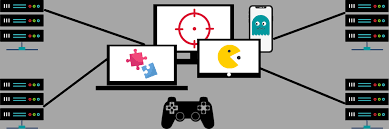
\includegraphics[width=0.8\textwidth]{PhotoMemoire/serveur_jeux.png}}
\caption{Un Schema de Serveur de Jeu}
	\end{figure}
\paragraph{ }
Un serveur de jeu est un type de serveur qui permet de fournir des services de jeu en ligne à des joueurs du monde entier. Les serveurs de jeu sont utilisés pour héberger des jeux multijoueurs en ligne, tels que les jeux de tir à la première personne, les jeux de stratégie en temps réel, les jeux de rôle en ligne massivement multijoueurs (MMORPG), les jeux de sport en ligne, etc.

Les serveurs de jeu offrent des fonctionnalités telles que :
\begin{enumerate}
	
  \item 1. Hébergement de jeux multijoueurs : Les serveurs de jeu sont utilisés pour héberger des jeux multijoueurs en ligne pour permettre aux joueurs de jouer ensemble sur Internet.
 
 \item  Gestion des joueurs : Les serveurs de jeu peuvent gérer les joueurs, les scores, les classements et les statistiques de jeu, ainsi que les opérations de modération pour assurer un environnement de jeu sécurisé et équitable.
 
 \item  Optimisation des performances : Les serveurs de jeu peuvent être optimisés pour offrir des performances de jeu optimales, telles que des temps de latence réduits et une faible latence pour une expérience de jeu fluide.
 
\item    Gestion de la bande passante : Les serveurs de jeu peuvent gérer la bande passante pour optimiser les performances de jeu et éviter les problèmes de lag ou de décalage.
 
 \item  Gestion des mises à jour : Les serveurs de jeu peuvent gérer les mises à jour de jeu pour maintenir les joueurs à jour avec les dernières fonctionnalités et correctifs de bugs.
 
\end{enumerate}

Les serveurs de jeu sont utilisés par les développeurs de jeux pour héberger leurs jeux en ligne et fournir des services de jeu en ligne à des millions de joueurs dans le monde entier. Les serveurs de jeu peuvent être exploités directement par les développeurs de jeux ou par des fournisseurs de services tiers spécialisés dans l'hébergement de serveurs de jeu. Les serveurs de jeu sont essentiels pour les jeux multijoueurs en ligne, car ils permettent aux joueurs de jouer ensemble sur Internet, offrant ainsi une expérience de jeu immersive et sociale.
 

Il existe plusieurs vulnérabilités potentielles qui peuvent affecter les serveurs de jeu. Voici quelques exemples :
\begin{enumerate}
\item   Vulnérabilités de sécurité : Les serveurs de jeu peuvent avoir des vulnérabilités de sécurité connues qui peuvent être exploitées par les attaquants pour accéder à des données sensibles, telles que des informations de compte de joueur ou des données de paiement.
	
	\item   Attaques par déni de service (DoS) : Les attaquants peuvent lancer des attaques par déni de service (DoS) contre le serveur de jeu pour le rendre indisponible, ce qui peut empêcher les joueurs d'accéder au jeu ou de jouer en ligne.
	
	\item   Exploits de jeu : Les attaquants peuvent exploiter des vulnérabilités dans le code du jeu pour gagner un avantage injuste sur les autres joueurs, ou pour perturber le jeu pour tous les autres joueurs.
	
	\item   Vulnérabilités de configuration : Les serveurs de jeu peuvent avoir des vulnérabilités de configuration qui peuvent être exploitées par les attaquants pour accéder à des données sensibles, telles que des informations de connexion ou des fichiers de configuration.
	
\item   Fuites de données : Les serveurs de jeu peuvent être vulnérables aux fuites de données, qui peuvent se produire lorsque des données sensibles sont stockées de manière inappropriée ou lorsque des utilisateurs non autorisés y ont accès.
\end{enumerate}

\paragraph{}
Il est important de mettre en place des mesures de sécurité adéquates pour protéger les serveurs de jeu contre ces vulnérabilités potentielles, telles que la mise à jour régulière de la sécurité du système et l'utilisation de logiciels de sécurité pour détecter et prévenir les attaques potentielles. Les développeurs de jeux doivent également être conscients des meilleures pratiques de sécurité, telles que la validation des entrées utilisateur et l'utilisation de l'authentification à deux facteurs pour protéger les comptes de joueur. Les administrateurs de serveurs de jeu doivent également surveiller les activités suspectes et mettre en place des politiques de sécurité strictes pour minimiser les risques d'attaques.

 \section*{\underline{Constat}}
 Si vous remarquez  bien que sur tout les serveurs que je viens de citer nous voyons que les attaques comme :
 \begin{enumerate}
 	\item L'Attaque Par Déni de Service (DoS).
 	\item Vulnérabilité de Configuration.
 	\item Fuites de données.
 	\item  Vulnérabilité de Sécurité  .
 \end{enumerate}
\paragraph{ }
Dans ce le chapitre qui suit nous allons essayer de parler des méthodes,  manières par lesquelles nous pouvons éviter de tomber  dans les pièges d'attaques citées ci-hauts .
